\documentclass[a4paper,11pt]{article}

\usepackage[utf8]{inputenc}
\usepackage{amsmath,amssymb,amsthm,mathrsfs,amsfonts,dsfont,bm} 
\usepackage[dvipsnames,table,xcdraw]{color,xcolor}
\usepackage{array,graphicx}
\usepackage{hyperref}
\usepackage{float, wrapfig}
\usepackage{empheq}
\usepackage[margin=2.5cm]{geometry}
\usepackage[toc]{appendix}
\usepackage{enumerate}
\usepackage{mathtools}  
\usepackage{multirow}
\usepackage{tikz}
\usepackage[round, sort]{natbib}
\usepackage{setspace}
\usepackage[affil-it]{authblk}
\usepackage[french,english]{babel}
\usetikzlibrary{shapes,backgrounds,arrows,automata,snakes,shadows,positioning, mindmap}

\newcommand{\edgeunit}{1.5}
\newcommand{\nodesize}{1em}
%\newcommand{\edgeunit}{4*\nodesize}
\newcommand{\length}{1}
\tikzstyle{covariate}=[draw, rectangle, minimum width=\nodesize, minimum height=\nodesize, inner sep=0, color=black]
\tikzstyle{covmiss}=[draw, minimum width=\nodesize, minimum height=\nodesize, inner sep=0, color=gray, text=gray]
\tikzstyle{observed}=[draw, circle, minimum width=\nodesize, inner sep=0, color=black]
\tikzstyle{edge}=[-, line width=1pt, color=black]
\tikzstyle{edgemiss}=[-, line width=1pt, dashed, color=gray]
\tikzstyle{variable}=[scale=0.9,rectangle,draw=white,transform shape,fill=white,font=\Large]
    

%%%%%%%%%%%%%%%%%%%%%%%%%%%%%%%%%%%%%%%%%%%%%
%% Environment
\renewcommand{\appendixname}{Annex}
\newtheorem{theorem}{Theorem}
\newtheorem{lemma}{Lemma}
\newtheorem{remark}{Remark}
\renewcommand{\abstractname}{Summary} 
\definecolor{red1}{RGB}{228,26,28}
\definecolor{red2}{RGB}{251,180,174}
\definecolor{blue1}{RGB}{55,126,184}
\definecolor{blue2}{RGB}{179,205,227}
\definecolor{aqua2}{RGB}{0,161,108}
\definecolor{aqua1}{RGB}{151,217,195}

 
\newcommand{\RM}[2]{\textcolor{aqua1}{\sout{#1}}\textcolor{aqua2}{#2}} % Raph
\newcommand{\SR}[2]{\textcolor{gray}{#1}\textcolor{blue}{#2}} % SR

\newcommand\independent{\protect\mathpalette{\protect\independenT}{\perp}}
\newcommand{\STAB}[1]{\begin{tabular}{@{}c@{}}#1\end{tabular}}

% Functions
\def\independenT#1#2{\mathrel{\rlap{$#1#2$}\mkern2mu{#1#2}}}
\DeclareMathOperator*{\argmax}{arg\,max}
\DeclareMathOperator*{\argmin}{arg\,min}
\DeclareMathOperator*{\Esp}{\mathbb{E}}
\DeclareMathOperator*{\Var}{\mathbb{V}}
\DeclareMathOperator*{\Cov}{\mathbb{C}\text{ov}}
\DeclareMathOperator*{\prob}{\mathds{P}}
\DeclareMathOperator*{\probt}{\widetilde{\mathds{P}}}

% Notations pairs
\newcommand\jk{{jk}}

% Notations cal
\newcommand\Ccal{\mathcal{C}}
\newcommand\Ncal{\mathcal{N}}
\newcommand\Pcal{\mathcal{P}}
\newcommand\Tcal{\mathcal{T}}
\newcommand\mt{\widetilde{m}}
\newcommand\St{\widetilde{S}}
\newcommand\mbt{\widetilde{\bf m}}
\newcommand\Sbt{\widetilde{\bf S}}

% Notations bf
\newcommand\gammab{{\boldsymbol{\gamma}}}
\newcommand\betab{{\boldsymbol{\beta}}}
\newcommand\thetab{{\boldsymbol{\theta}}}
\newcommand\Sigmab{{\boldsymbol{\Sigma}}}
\newcommand\cst{\text{cst}}
\newcommand\Ob{{\bf O}}
\newcommand\Hb{{\bf H}}
\newcommand\Mb{{\bf M}}
\newcommand\Qb{{\bf Q}}
\newcommand\Wb{{\bf W}}
\newcommand\Xb{{\bf X}}
\newcommand\xb{{\bf x}}
\newcommand\Yb{{\bf Y}}
\newcommand\Zb{{\bf Z}}
\newcommand\zb{{\bf z}}



% Notations tilde
\newcommand\Pt{\widetilde{P}}
\newcommand\pt{\widetilde{p}}
\newcommand\et{\widetilde{\mathds{E}}}
\newcommand\e{{\mathds{E}}}
% TikZ
\newcommand{\nodesize}{1em}
\newcommand{\edgeunit}{4*\nodesize}
\tikzstyle{covariate}=[draw, rectangle, minimum width=\nodesize, minimum height=\nodesize, inner sep=0, color=black]
\tikzstyle{covmiss}=[draw, minimum width=\nodesize, minimum height=\nodesize, inner sep=0, color=gray, text=gray]
\tikzstyle{observed}=[draw, circle, minimum width=\nodesize, inner sep=0, color=black]
\tikzstyle{edge}=[-, line width=1pt, color=black]
\tikzstyle{edgemiss}=[-, line width=1pt, dashed, color=gray]

\newcommand{\argmin}{\arg\!\min}
\newcommand{\argmax}{\arg\!\max}
\newcommand*\widefbox[1]{\fbox{\hspace{3em}#1\hspace{3em}}}
\newcommand*\lesswidefbox[1]{\fbox{\hspace{2em}#1\hspace{2em}}}
\newcommand{\entr}{\mathcal{H}}
\newcommand{\betabf}{\boldsymbol{\beta}}
\newcommand{\thetabf}{\boldsymbol{\theta}}
\newcommand{\mubf}{\boldsymbol{\mu}}
\newcommand{\Omegabf}{\boldsymbol{\Omega}}
\newcommand{\Sigmabf}{\boldsymbol{\Sigma}}
\newcommand{\zerobf}{\boldsymbol{0}}
\newcommand{\Xbf}{\boldsymbol{X}}
\newcommand{\xbf}{\boldsymbol{x}}
\newcommand{\Ybf}{\boldsymbol{Y}}
\newcommand{\Zbf}{\boldsymbol{Z}}
\newcommand{\Sbf}{\boldsymbol{S}}
\newcommand{\mbf}{\boldsymbol{m}}
\newcommand\Ncal{\mathcal{N}}
\newcommand\Pcal{\mathcal{P}}
\newcommand\Tcal{\mathcal{T}} 
\newcommand{\Esp}{\mathds{E}}
\newcommand{\bound}{\mathcal{J}}

\definecolor{coquelicot}{rgb}{1.0, 0.22, 0.0}
\newcommand{\modifRM}[1]{\textcolor{coquelicot}{#1}}
\newcommand{\modifSR}[2]{\textcolor{gray}{#1}\textcolor{blue}{#2}}
%%%%%%%%%%%%%%%%%%%%%%%%%%%%%%%%%%%%%%%%%%%%%

\title{\textbf{Prise en compte d'un acteur manquant dans l'inférence de réseaux d'interactions d'espèces par mélange d'arbres à partir de données de comptages}}

\author{Raphaëlle Momal$^1$%
  \thanks{Electronic address: \texttt{raphaelle.momal@agroparistech.fr}; Corresponding author}, \hspace{0.3cm} Stéphane Robin$^1$, \hspace{0.3cm} Christophe Ambroise$^2$}
\affil{1: Université Paris-Saclay, AgroParisTech, INRAE, UMR MIA-Paris, Paris, France.\\
2: Laboratoire de Mathématiques et Modélisation d'Évry, 23 bvd de France, Évry, France}

\date{\vspace{-5ex}}
%\date{\today}

\begin{document}
\setlength{\parindent}{0ex}
\maketitle
%%%%%%%%%%%%%%%%%%%%%%%%%%%%%%%%%%%%%%%%%%%%%
 

\selectlanguage{english}
\begin{abstract}
Network inference is used in many areas such as genomics or ecology to infer the structure of conditional independence between covariates, based on the measures of gene expression or species abundance for example. In many experiments, it is likely that not all covariates involved in the network were actually observed. Then observed samples are drawn from a distribution where some unobserved covariates were marginalized.

We introduce a generic staitstical model for network inference from abundance data with missing actor. The model includes fixed effects to take account of environmental covariates  and sampling efforts, as well as correlated random effects to encode species interactions. The correlation structure is that of a gaussian graphical model marginalized on one ore more covariates, corresponding to the missing actors. The inferred network is obtained by averaging on all spanning trees, in a computationnally efficient way.
\paragraph{Key-words: }  graphical models, network inference, missing actor, abundance data, Variational EM algorithm, matrix tree theorem, Poisson log-Normal model
\end{abstract}
 
% intro
%Les réseaux :
%- [ ] C’est quoi
%- [ ] À quoi ça sert (les enjeux, appliqué)
%- [ ] Quelles sont les questions qui se posent (que dit la recherche)
%
%- [ ] Lauritzen pour les nuls
%
%L’inférence de réseaux :
%- [ ] Quelle méthode pour quel réseau
%- [ ] Auxquelles on se compare, pourquoi elles sont comme ça comment elles marchent et ce qui manque

  \section*{Biological context}
 \subsection*{Networks}
 A network is an intuitive object which anyone can easily relate to. It is first of all a graphical tool representing the links between different entities. This helps understand how a system organizes and have a direct image of it. It is also an analysis tool which can unravel sensible information about the system, its structure and the different roles in its organization. Networks are versatile tools that are  used in many domains (e.g. sociology, linguistics, computer sciences, neurosciences, climatology, psychology, etc.) and can take various forms to adapt to each problem.  They can be directed or undirected. Some link entities with multiple kinds of edges (multidimensional), or have different layers (multiplex), others link groups of disconnected objects (multipartite). In biology, the most typical networks simply represent the species (nodes) and their relationships (edges).

Various types of species interactions are studied with networks. For example, their is a rich literature of networks for plant-pollinator and host-parasite relationships in ecology. These species interactions are clearly defined and directly observed in the field. Contacts of pollination or parasitism are counted and networks constructed from these interaction abundances.
\begin{figure}
\centering
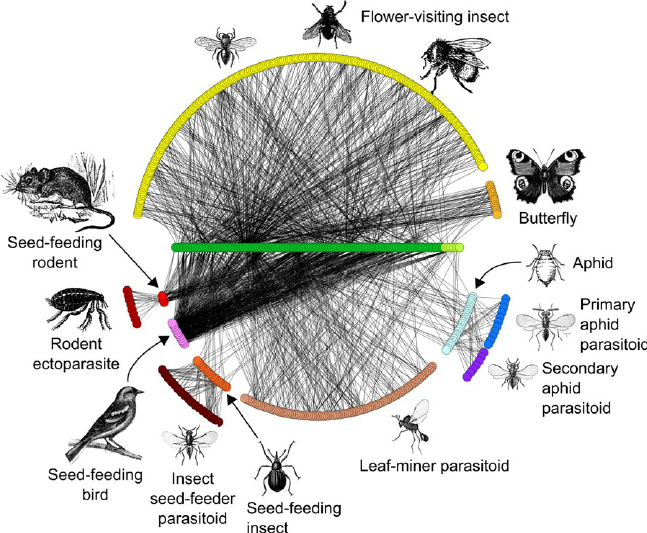
\includegraphics[width=0.7\linewidth]{figs/pocock.png}
\caption{Species interaction networks at Norwood Farm, Somerset, UK \citep{PED12,BRM13}.}
\label{pocock}
\end{figure}
 However many mechanisms cannot be observed and may not be well defined. One way to discover them may then be to resort to a more mathematical definition of species interactions. Working with the latter allows the study of community assembly mechanisms with the inference of networks representing guilds of species in community ecology. This type of network is extensively used in genomics for protein-protein interaction network, or gene regulatory networks, or in microbiology to study the output of a metabarcoding experiment assessing the composition of a microbiome. 
 
 \begin{figure}
\centering
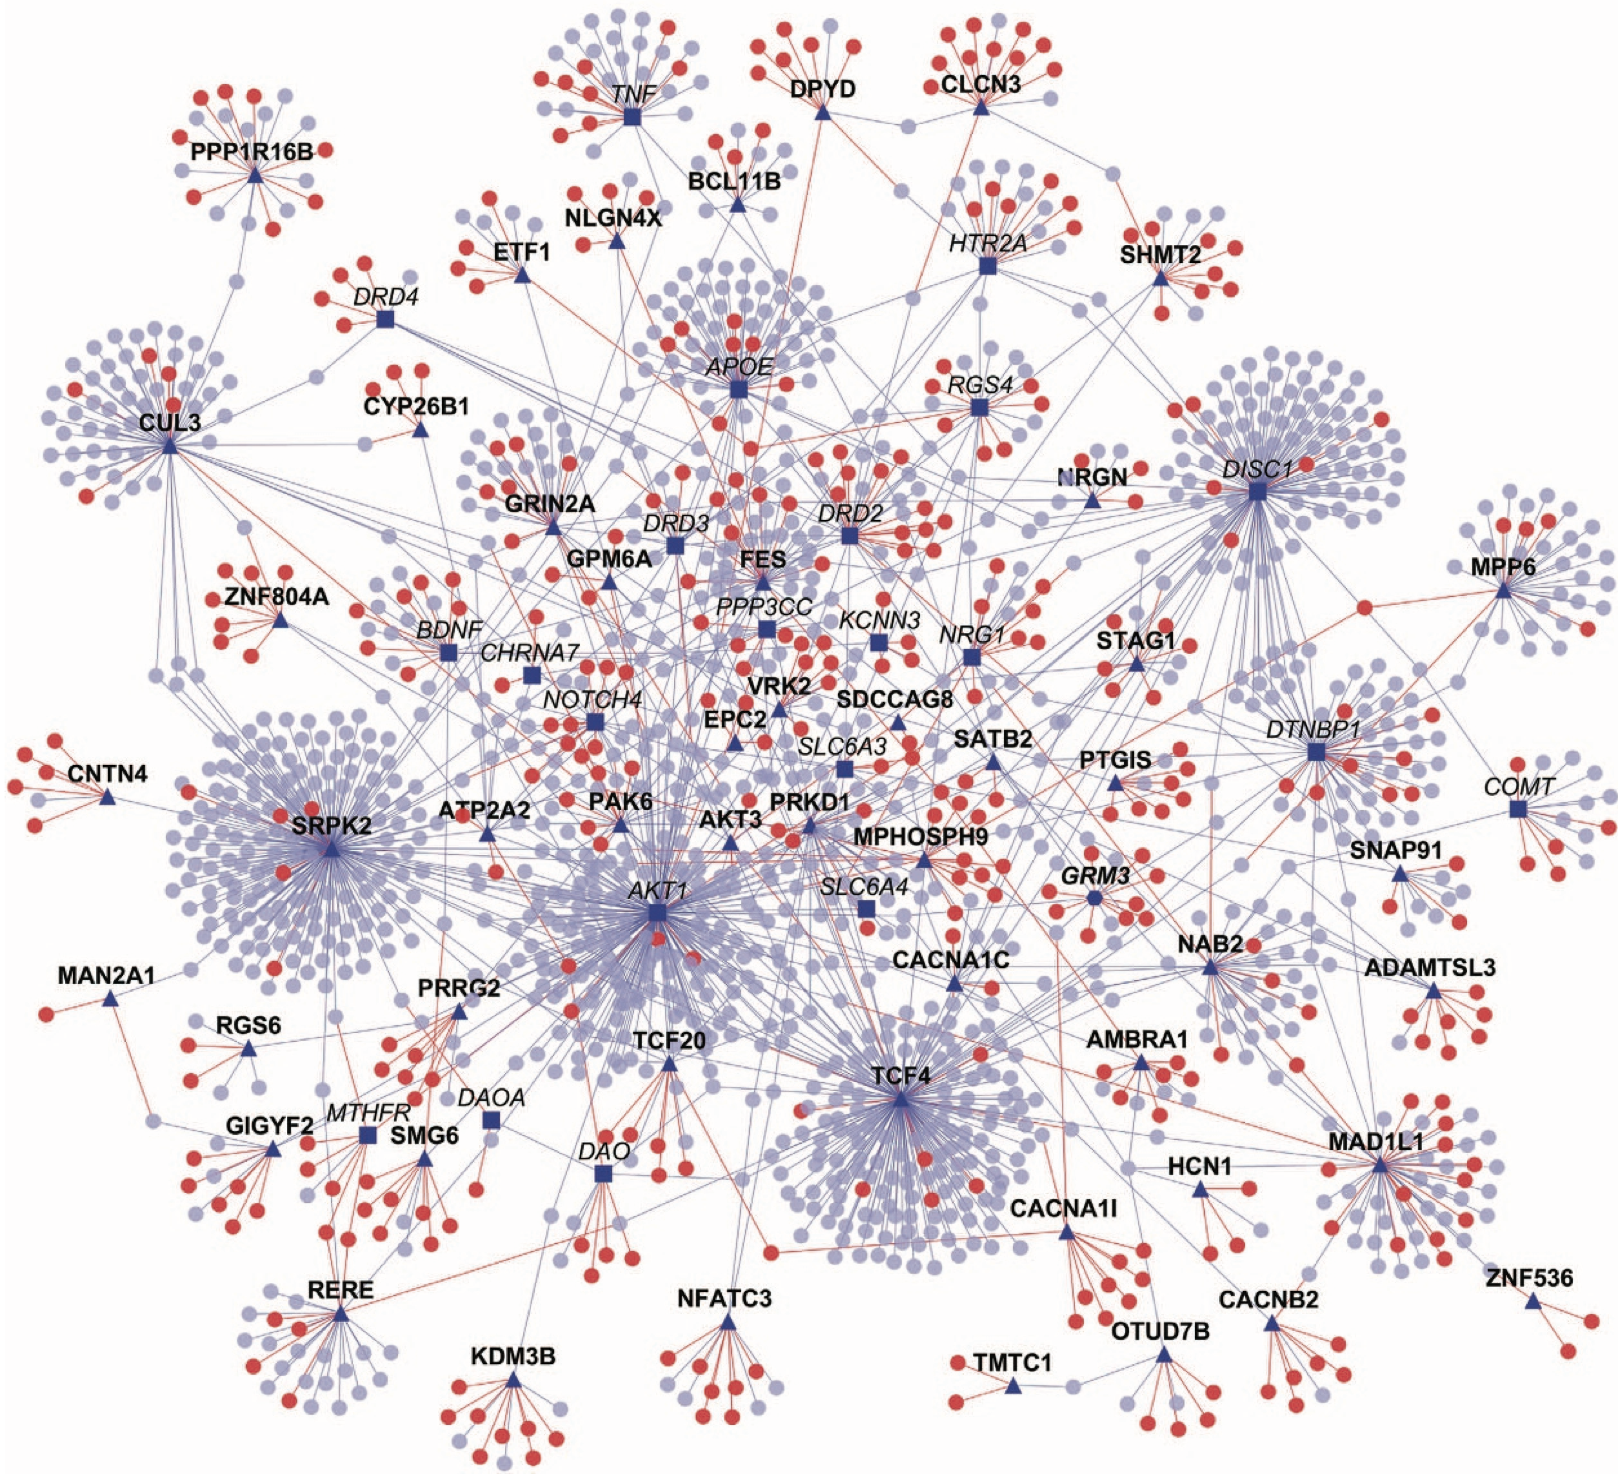
\includegraphics[width=0.7\linewidth]{figs/PPInetwork.png}
\caption{Protein-protein interactions between genes involved in schizophrenia \citep{GTH16}.}
\label{PPI}
\end{figure}

  \subsection*{Statistical interactions}
The correlations between the species measures first come to mind as a statistical characterization of an interaction. These are easily obtained, yet their corresponding networks are hard to interpret. Indeed, two covariates correlating with a same third one will appear correlated, even if they have no direct effect on each other\footnote{e.g. the number of covid 19 cases detected correlates with both the real number of cases and the number of tests done on the population, which induces a spurious correlation between the two latter where obviously there is no direct effect of one on the other.}. This phenomena of spurious correlations complicates both the analysis and the interpretation by inducing a very high number of edges  which cannot be categorized as direct or indirect associations between the species. 
 
 Conditional dependencies are then very useful measures of interaction. They describe dependencies between each pair of species conditional on all others. That is, all other species measures kept fixed, their measures should still be correlated. A link between two species can then be interpreted as a direct association. This yields a network of species conditional dependence (link) and independence (absence of link), which is interpretable and falls within the well-studied mathematical framework of graphical models.
 
 \subsection*{Measures on species}
 Networks of statistical interactions are obtained from datasets of repeated measures on a set of species, which can be of various types. Measures can be continuous, as for example the output of gene expression profiling experiments using DNA microarrays, which  are  fluorescences measures from targeted genes. Using a Gaussian approximation, these measures of genes expressions can be used to derive genes regulatory networks.  Measures can also be binary, as in co-occurrence data in ecology, which record the joint presences and absences of a set of species in several sites. \citet{CAM16}.
%développer les données de co-occurence

Abundance data  are joint counts of species in a series of sites (also known as assemblages data in ecology). Recent technologies made this type of data increasingly available. Assemblages data were rare in ecology as they implied intensive sampling efforts, which is now greatly facilitated by camera traps and sensors. In metagenomics, high-throughput sequencing technologies for metabarcoding experiments made it possible  to get joint counts of pseudo-species (operational taxonomic units (OTUs)) abundances.  Both domains work with the same type of output: a dataset of joint (pseudo-)species abundances from different sites or samples.\\
%développer les metabarcoding et OTU


Once the data has been collected, it is very likely that not all species or covariates were observed: there exists missing actors and data is incomplete. In the network, the existence of a missing actor translates into appearance of edges between all the species it should connect with, creating dense cliques of species which are not actually conditionally dependent on one another. A second objective of this work is to take missing actors into account during network inference in order to get more accurate interpretations.

\section*{Network inference}
% ce qui existe et motivation du sujet
\section*{Objectives}
 \subsection*{Graphical models and Trees}
The dedicated framework for the representation of conditional dependency structures are graphical models. Gaussian Graphical Models (GGM) in particular provide with appealing algebraic properties for network inference, which are detailed in \citet{Lau96}. Exploring the set of possible graphs is a non-ending task, and we chose to reduce the searching space to that of spanning trees. This is the sparsest connected structure, and enjoys specific algebraic properties allowing to sum on all possible spanning trees at the cost of a determinant calculus. Our network inference methodology relies on spanning trees and \citet{Lau96} maximum likelihood estimators for multivariate Gaussian graphical models.

%caser le missing actor qq part
 \subsection*{Modeling abundance data}
 As this ideal framework of GGM is not directly applicable to abundance data, there exist two possible ways to proceed: either apply a Gaussian transformation to the data, or rely on Gaussian latent vectors in the framework of Joint Species Distribution Models (JSDM). Our methodology resorts to the latter, and more specifically to the Poisson log-normal distribution to model the counts. This distribution allows easy handling of both covariates and offsets, as well as take overdispersion into account thanks to its Gaussian random parameters. 
 
 
 \subsection*{Estimation procedure} %or algorithm
The central model we adopt involves a Gaussian layer of parameters which is a mixture on all spanning trees. Each component of the mixture is a Gaussian distribution which dependency structure is a spanning tree. This represents two hidden layers of parameters, which we first estimates with an Estimation-Maximization (EM) algorithm. Then to infer missing actors of the network, we resort to a variational (VEM) approach.

\section*{Outline} 
  \subsection*{Chapter 1}
The first chapter details the mathematical tools and technical results for the statistical modeling and the network inference used in Chapters 2 and 3.

   \subsection*{Chapter 2}
   This chapter details a method to infer undirected networks representing conditional statistical dependencies between the species from their joint abundance measures.  The proposed methodology, implemented in the R package \texttt{EMtree},  is compared to state of the art approaches and applied to two empirical datasets from ecology and metagenomics. This chapter has been published as an article in the journal \textit{Methods in Ecology and Evolution} \citep{MRA20}.
   
    \subsection*{Chapter 3}
This chapter details a variational approach to the inference of a missing actor in the network. The reconstruction of missing actor(s) is implemented in the R package \texttt{nestor} and illustrated on two  empirical datasets from ecology. This chapter has been submitted for publication in the \textit{Journal of the Royal Statistical Society: series C (applied statistics)}.
 
  \subsection*{Chapter 4}
This final chapter introduces some natural perspectives of this work. After concluding on the specifics of the developed methodology, natural extension are presented, including network comparison. The inclusion of spatialized data is discussed, as well as the possibility of network inference directly from the observed counts.
 \section*{Notations}
 
 \begin{description}
 \item[Operations:]  \begin{itemize}
     \item[]
 \item[] $|\cdot|$ : matrix determinant
 \item[] $\odot$ : Hadamard product
 \end{itemize}
 \item[Variables:] \begin{itemize}
     \item[]
 \item[] $\Ybf$ :  matrix  of observed counts
 \item[] $\Zbf$ : matrix of latent Gaussian parameters 
 \item[] $\Ubf$ : matrix of latent normalized Gaussian parameters 
 \item[] $\Xbf$ : matrix of covariates 
 \item[] $O$ : matrix of measured offsets
 \end{itemize}
 \item[Dimensions:]\begin{itemize}
     \item[]
 \item[] $n$ : number of samples
 \item[] $p$: number of observed species
 \item[] $r$: number of unobserved species
 \item[] $d$: number of covariates
 \end{itemize}
 \end{description} 
Let us first describe the typical type of data we consider. We assume that $p$ species have been observed in $n$ sites. \validSR{The abundances are gathered in the $n \times p$ matrix $\Yb$. $Y_{ij}$ is the abundance of species $j$ in site $i$, and  $\Yb_i$ the abundance vector collected in site $i$ ($i$th row of $\Yb$).} We further assume that a vector of covariates $\xb_i$ \validSR{of size $d$} has been measured in each site $i$ and that all covariates are gathered in the $n \times d$ matrix $\Xb$. The sites are supposed to be independent.

Our aim is to decipher the dependency structure between the $p$ species, accounting for the effect of the environmental covariates encoded in $\Xb$. As explained above, ignoring environmental covariates is more than likely to result in spurious edges. 

\paragraph{Mixed model.}
To distinguish between covariates effects and species interactions, we consider a mixed model which states that each abundance $Y_{ij}$ has a (conditional) Poisson distribution
 
\begin{equation} \label{eq:pY.Z}
    Y_{ij} \sim \Pcal\left(\exp(\xb_i^\intercal \thetab_j + o_{ij} + Z_{ij})\right).
\end{equation}
 
In model (\ref{eq:pY.Z}), $o_{ij}$ is the sample- and species-specific offset which accounts for the sampling effort. $\thetab_j$ is the vector of fixed regression coefficients measuring the effect of each covariate on species $j$ abundance. The regression part is similar to a general linear model as used in niche modeling \citep[see e.g.][]{austin2007species}. 
\modif{$Z_{ij}$ is the random effect associated with species $j$ in site $i$. 
Importantly, the coordinates of the site-specific random vector $\Zb_i = (Z_{i1}, \dots Z_{ip})$ are not independant: the multivariate random term $\Zb_i$ precisely accounts for the interactions that are not due to environmental fluctuations. 
For each site $i$, a vector $\Zb_i$ is associated with the corresponding abundance vector $\Yb_i$.}
The distribution given in Eq.~\eqref{eq:pY.Z} is over-dispersed as the Poisson parameter is itself random, which suits ecological modeling of abundance data \citep{Eco_overdisp}.

\bigskip
We now describe the distribution of the latent vector $\Zb_i$. To this aim, we adopt a version of Kirshner's model \citep{kirshner}, which states that a spanning tree $T$ is first drawn with probability
 
\begin{equation} \label{eq:pT}
    p(T) = \prod_{(j, k) \in T} \beta_{jk} / B,
\end{equation}
 
where $(j, k) \in T$ means that the edge connecting species $j$ and $k$ is part of the tree $T$ and where $B$ is a normalizing constant. Each edge weight $\beta_{jk}$ controls the probability for the edge $(j, k)$ to be in the interaction network. \\
Then for each site $i$, a vector $\Zb_i$ is drawn independently with conditional Gaussian distribution $(\Zb_i \mid T) \sim \Ncal(0, \Sigma_T)$, where the subscript T means that the distribution of $\Zb_i$ is {faithful} to $T$. When $T$ is a spanning tree, this faithfulness simply means this distribution can be factorized on the nodes and edges of $T$ as follows \citep[see][]{kirshner}:
 
\begin{equation} \label{eq:pZfact}
p(\Zb_i \mid T) = \prod_{j=1}^p p(Z_{ij}|T) \prod_{(j, k) \in T} \psi_{jk}(\Zb_i),
\end{equation}
 
where $\psi_{jk}(\Zb_i)$ does not depend on $T$. This factorization means that each edge of $T$ corresponds to a species pair in direct interaction;  all other pairs are conditionally independent. Experiments are independent, and in the sequel we consider the product of all $p(\Zb_i)$ and use the simpler notation $\psi_{jk} = \prod_i \psi_{jk}(\Zb_i)$ instead.\\

According to Eq.~\eqref{eq:pT}, each $\Zb_i$ has a Gaussian distribution conditional on the tree $T$, so its marginal distribution is a mixture of Gaussians: $\Zb_i \sim \sum_{T \in\mathcal{T}} p(T) \Ncal(0, \Sigma_T)$, where $\mathcal{T}$ is the set of all spanning trees. As a consequence, the joint distribution of the $\Zb_i$ is modeled by a mixture of distributions with tree-shaped dependency structure. \\
Besides, for all trees including the edge $(j, k)$, the estimate of the covariance term between the coordinates $j$ and $k$ is the same \citep[see][]{Lau96,SRS19}. Hence, we may define a global covariance matrix $\Sigmab$, filled with covariances that are each common to spanning trees containing a same edge. Each $\Sigmab_T$ is then built by extracting from $\Sigmab$ the covariances corresponding to the edges of $T$.

%%%%%%%%%%%%%%%%%%%%%%%%%%%%%%%%%%%%%%%%%%%%%%%%%%%%%%%%%%%%%%%%%%%%%%%%%%%%%%%%
\section{Inference} \label{sec:Inference}
%%%%%%%%%%%%%%%%%%%%%%%%%%%%%%%%%%%%%%%%%%%%%%%%%%%%%%%%%%%%%%%%%%%%%%%%%%%%%%%%

As said in the introduction, we  resort to a variational EM algorithm to perform the inference due to the complex latent structure.

%%%%%%%%%%%%%%%%%%%%%%%%%%%%%%%%%%%%%%%%%%%%%%%%%%%%%%%%%%%%%%%%%%%%%%%%%%%%%%%%%%%%%%%
\subsection{Variational inference}
%%%%%%%%%%%%%%%%%%%%%%%%%%%%%%%%%%%%%%%%%%%%%%%%%%%%%%%%%%%%%%%%%%%%%%%%%%%%%%%%%%%%%%%

The log-likelihood of the so-called {\sl complete} data, that is $(\Ybf, \Ubf, T)$, writes
\begin{align*}
\log p_{\thetabf, \betabf, \Omega}(\Ybf, \Ubf, T) 
& = \log p_\betabf(T) + \log p_{\Omegabf}(\Ubf \mid T) + \log p_\thetabf(\Ybf \mid \Ubf).
\end{align*}
where $\Omegabf$ stands for the set of all tree-specific precision matrices: $\Omegabf = \{\Omegabf_T, T \in \Tcal_{p+r}\}$.
The conditional distributions of the latent variables $\Ubf$ and of the tree $T$ given the data $\Ybf$ are both intractable. Variational inference then aims at maximizing a lower bound of the log-likelihood of the observed data, which writes in our context as
\begin{align} \label{eq:lower-bound}
\Jcal(\thetabf, \betabf, \Omega; q)
& = \log p_{\thetabf, \betabf, \Omega}(\Ybf) 
- KL\left(q(\Ubf, T) \| p_{\thetabf, \betabf, \Omega}(\Ubf, T \mid \Ybf) \right) \\
& = \Esp_q \log p_{\thetabf, \betabf, \Omega}(\Ybf,\Ubf, T) + \Hcal(q(\Ubf, T)), \nonumber
\end{align}
where $q(\Ubf,T)$ stands for the approximate joint conditional distribution of the latent layer and of the tree: $q(\Ubf, T) \simeq p(\Ubf, T \mid \Ybf)$. 

%%%%%%%%%%%%%%%%%%%%%%%%%%%%%%%%%%%%%%%%%%%%%%%%%%%%%%%%%%%%%%%%%%%%%%%%%%%%%%%%%%%%%%%
\subsubsection*{Approximate distribution.}
The efficiency of variational inference mostly depends on the choice of $q(\Ubf, T)$, which is a balance between computational ease and adequation to the target distribution $p(\Ubf, T \mid \Ybf)$. We adopt here a classical product form for the approximate distribution: we impose to the latent variables $\Ubf$ and to the tree $T$ to be independent according to $q$ (whereas actually they are not conditional on the data), with respective marginals $h$ and $g$:
$$
q(\Ubf, T) =  h(\Ubf)g(T).
$$
Because the sites are independent, and without further assumption, the distribution $h$ is a product over all sites. Following \cite{CMR18} we approximate the conditional distribution of each latent vector $\Ubf_i$ with a Gaussian distribution, that is:
$$
h(\Ubf) = \prod_i \Ncal_{p+r}(\Ubf_i; \mbf_i, \Sbf_i).
$$
with all $\Sbf_i$ diagonal. We gather all the mean vectors $\mbf_i$ in the $n \times (p+r)$ matrix $\Mbf$ and pile up the diagonals of all the variance matrices $\Sbf_i$ in the $n \times (p+r)$ matrix denoted $\Sbf$.

%%%%%%%%%%%%%%%%%%%%%%%%%%%%%%%%%%%%%%%%%%%%%%%%%%%%%%%%%%%%%%%%%%%%%%%%%%%%%%%%%%%%%%%
\subsubsection*{Variational EM.}
The variational EM algorithm then consists in maximizing the lower bound $\Jcal$ defined in \eqref{eq:lower-bound} with respect to the parameters (M step), and to the approximate distributions (VE step), alternatively. 
\begin{description}
\item[M step:] At iteration $t+1$, given the current approximate distribution $q^t(\Ubf, T) = g^t(T) h^t(\Ubf)$, the M step consists in the update of the model parameters, solving 
\begin{align} \label{eq:Mstep}
\thetabf^{t+1} & = \arg\max_\thetabf \; \Esp_{h^t} \left[ \log p_\thetabf(\Ybf \mid \Ubf) \right], 
& \Omegabf^{t+1} & = \arg\max_\Omegabf \; \Esp_{q^t} \left[ \log p_{\Omegabf}(\Ubf \mid T) \right], \nonumber \\
\betabf^{t+1} & = \arg\max_\betabf \; \Esp_{g^t} \left[ \log p_\betabf(T) \right].
\end{align}
Observe that the matrix of edge weights $\betabf$ is considered here as a parameter to be estimated, as opposed to \cite{RAR19}, where it was kept fixed and supposed to be given.
%
\item[VE step:] Maximising $\Jcal$ with respect to (wrt) $q$ is equivalent to minimizing the K\"ullback-Leibler divergence between $q(\Ubf, T)$ and $p_{\thetabf, \betabf, \Omega}(\Ubf, T \mid \Ybf)$ that appears in \eqref{eq:lower-bound}. Because we adopted a product form for $q$, the solution of the VE step for both $g$ and $h$ is known to be a mean-field approximation \citep{WaJ08}. More specifically, maximising $\Jcal$ gives
\begin{align} \label{eq:VEstep-g}
g^{t+1}(T) 
& \propto \exp \left\{ \Esp_{h^t} \left[ \log p_{\thetabf^{t+1}, \betabf^{t+1}, \Omega^{t+1}}(\Ybf, \Ubf, T) \right] \right\} \nonumber \\
& \propto \exp \left\{ \log p_{\betabf^{t+1}}(T) + \Esp_{h^t} \left[ \log p_{\Omegabf^{t+1}}(\Ubf \mid T) \right] \right\},
\end{align}
and
\begin{align} \label{eq:VEstep-hH}
h^{t+1}(\Ubf) 
& \propto \exp \left\{ \Esp_{g^{t+1}} \left[ \log p_{\thetabf^{t+1}, \betabf^{t+1}, \Omega^{t+1}}(\Ybf, \Ubf, T) \right] \right\} \nonumber \\
& \propto \exp \left\{ \Esp_{g^{t+1}} \left[ \log p_{\Omegabf^{t+1}}(\Ubf \mid T) \right] + \log p_{\thetabf^{t+1}}(\Ybf \mid \Ubf) \right\}. 
\end{align}
\end{description}

Observing that $\log p_\betabf(T) + \log p_{\Omegabf}(\Ubf \mid T)$ can be written as a sum over all the edges present in $T$, we see that $g^{t+1}(T)$ has a product form. So, without any further assumption, we may parametrize $g(T)$ in the same way as $p_\betabf(T)$:
\begin{equation} \label{eq:g}
g(T) = \prod_{jk \in T} \betat_{jk} / \Bt
\qquad \text{where} \quad
\Bt = \sum_{T \in \Tcal_{p+r}} \prod_{jk \in T} \betat_{jk}.
\end{equation}
We gather the $\betat_{jk}$'s in the $(p+r) \times (p+r)$ matrix $\betabft$. The parameters $\betabft$, $\Mbf$ and $\Sbf$ are called the variational parameters, in the sense that it is equivalent to optimize $\Jcal$ wrt $(g, h)$ or wrt $(\betabft, \Mbf, \Sbf)$.

%%%%%%%%%%%%%%%%%%%%%%%%%%%%%%%%%%%%%%%%%%%%%%%%%%%%%%%%%%%%%%%%%%%%%%%%%%%%%%%%%%%%%%%
\subsection{Proposed algorithm}
\label{algo}
%%%%%%%%%%%%%%%%%%%%%%%%%%%%%%%%%%%%%%%%%%%%%%%%%%%%%%%%%%%%%%%%%%%%%%%%%%%%%%%%%%%%%%%

The model we consider is an extension of the PLN model, for which an efficient inference algorithm have been implemented in \url{PLNmodels}, an R package available on CRAN \citep{CMR18,CMR19}. 

\subsubsection*{Prior estimates of $\thetabf$, $\Mbf_O$ and $\Sbf_O$.}
To alleviate the computational burden of the inference, we take advantage of this available tool to get an estimate of the regression coefficient matrix $\widehat{\thetabf}$ and an approximation of the parameters  of the observed latent variable conditional distribution $h_O(\Ubf_O) \simeq p(\Ubf_O \mid \Ybf)$. These latter parameters are $\Mbf_O$ and $\Sbf_O$ (first $p$  columns of $\Mbf$ and $\Sbf$ respectively) and we denote $\Mbft_O$ and $\Sbft_O$ their approximation. The quantities $\widehat{\thetabf}$, $\Mbft_O$ and $\Sbft_O$ are kept fixed in the rest of the algorithm, so the VEM algorithm only deals with the remaining unknown quantities: the model parameters $\betabf$, $\Omegabf$, and the variational parameters $\betabft$, $\Mbf_H$, $\Sbf_H$. 
% \textcolor{red}{[on ne dit plus que c'est sous-optimal ? "optimal value for MO and SO" est un peu fort ?]}
As a consequence, the final estimates we get yield a lower value of the objective function $\Jcal$ as compared to  an optimisation wrt all model and variational parameters.

%%%%%%%%%%%%%%%%%%%%%%%%%%%%%%%%%%%%%%%%%%%%%%%%%%%%%%%%%%%%%%%%%%%%%%%%%%%%%%%
\subsubsection*{M step.} This step deals with the update of the  model parameters $\betabf$ and $\Omegabf_T$. Some of the calculations are tedious and postponed to Appendix \ref{app:comput}.

\paragraph{Edges weights $\betabf$:} 
As shown in Equation \eqref{eq:Mstep}, the maximization of $\mathcal{J}$ requires the computation of the derivative of $\Esp_{g^t} [\log p_{\betabf}(T)]$ wrt $\betabf$, which includes the derivative of the normalizing constant $B$. The latter can be computed via an extension of the Matrix Tree theorem \citep[see][Lemma \ref{lem:Meila} reminded in Appendix \ref{app:tools}]{MeilaJaak}. Setting the derivative of the expectation to 0 yields the following update (same as in \citet{MRA20} and detailed in appendix \ref{up:beta}):
$$
\beta^{t+1}_{kl} 
= \frac{P^t_{kl}}{ M(\betabf^t)_{kl}},
$$
where $M(\betabf)$ is defined in Lemma \ref{lem:Meila} and $P^t_{kl}$ is the probability that the edge $(k, l)$ belongs to the tree $T$ according to $g^t$:
$$
P^t_{kl} = \mathds{P}_{g^t}\{kl \in T\} 
= \sum_{\substack{T  \in \mathcal{T}: \\ T \ni kl}} g^t(T) 
= \frac{1}{\Bt^t} \sum_{\substack{T  \in \mathcal{T}: \\ T \ni kl}} \prod_{uv \in T} \betat^t_{uv}.
$$
$P^t_{kl}$ is computed using a result from \citet{kirshner} (reminded as Lemma \ref{lem:Kirshner} in appendix A). We now define the binary variable $I_{Tkl}$ which indicates the presence of the edge $kl$ in tree $T$, so $P_{kl}^t = \Esp_{g^t} [I_{Tkl}]$ and $I_T = [I_{Tkl}]_{1 \leq k, l \leq (p+r)}$ is the adjacency matrix of tree $T$.

\paragraph{Precision matrices $\Omegabf_T$:}
For a given dependency structure in the Gaussian Graphical model framework, \cite{Lau96} gives maximum likelihood estimates for the precision matrix. 
These estimators are given as functions of sufficient statistics of the multivariate Gaussian distribution. Indeed in the exponential family framework, the M step of any EM algorithm requires the computation of the expectation of a sufficient statistic, under the current fit of the variational laws (see \citet{mclachlan}). Here as $\Ubf \mid T$ is centered, a sufficient statistic is $\Ubf^\intercal \Ubf$. We now let $SSD$ denote the matrix defined as 
$$
SSD^t = \Esp_{h^t} (\Ubf^\intercal \Ubf) = (\Mbf^t)^\intercal \Mbf^t + \Sbf^t_+,
$$
where $\Sbf^t_+ = \sum_i \Sbf^t_i$. Applying Lauritzen's formulas, we get:
%As $g^t$ is a discrete law on the space of spanning trees, maximizing each component of an expectation wrt $g$ amounts to  maximizing the whole expectation, meaning that maximizing for each tree $T$ will maximize $\mathcal{J}(\Ybf ; g,h)$.
%The off-diagonal and diagonal terms of $\hat{\Omega}_T$ write as follows with normalized data:
\begin{align} \label{omegaT}
\omega^{t+1}_{Tkl} & = \left\{
\begin{array}{ll}
\dfrac{ -ssd_{kl}^{\,t}/n}{1-(ssd_{kl}^{\,t}/n)^2} & \text{if } kl \in T \\
0 & \text{otherwise}
\end{array} 
\right., \\
\omega^{t+1}_{Tkk} & = 1 + \sum_l I_{Tkl} \dfrac{(ssd_{kl}^{\,t}/n)^2}{1-(ssd_{kl}^{\,t}/n)^2},
\nonumber
\end{align}
where $ssd^t_{kl}$ stands for the entry $kl$ of the matrix $SSD^t$.
The calculations are postponed to Appendix \ref{up:omega}. Observe that estimates of the off-diagonal entries $\omega^{t+1}_{Tkl}$ do not depend on $T$ provided that the edge $(k, l)$ belongs to $T$.  Thus the estimates of the off-diagonal terms of the precision matrices $\Omegabf_T$ are common to all trees sharing a given edge. This does not result from any assumption on the shape of  $\Omegabf_T$, but from the properties of the maximum likelihood estimate of Gaussian variance matrix. In the sequel we will simply denote off-diagonal terms by $\omega_{kl}$ (as opposed to $\omega_{Tkk}$ which still depends on $T$).\\

Other quantities are needed for later computations. Lauritzen  gives the maximum likelihood estimator of every entry of the correlation matrix $\Rbf_T$ corresponding to an edge $kl$ being part of $T$, which is
$ \Rbf_{Tkl}^{t+1} = ssd_{kl}^{\,t}/n. $
Hereafter for any matrix $A$, $A_{[kl]}$ refers to the bloc $kl$ of $A$: $A_{[kl]}=(a_{ij})_{\{i,j\}\in\{k,l\}}$. The determinant of $\Omegabf^{t+1}_T$ factorizes on the edges of $T$ and writes as a function of blocks of the correlation matrix  as follows:  

\begin{align}
    |\Omegabf^{t+1}_{T}| = \Big(\prod_{kl \in T} |\Rbf_{T[kl]}^{t+1}|\Big)^{-1}
\quad 
\text{and for any $kl \in T$, } 
|\Rbf_{T[kl]}^{t+1}|= 1-(ssd_{kl}^{\,t}/n)^2. \label{RT}
\end{align}

 
Finally we define the matrix  $\xbar{\Omegabf}^{\,t+1} = \Esp_{g^t}[\Omegabf^{t+1}_T]$. 
%\CA{By definition of the $I_T$ matrix,  off-diagonal and diagonal terms of $\xbar{\Omegabf}$ make edges probabilities appear as follows}
Noticing that, for $k \neq l$, $\Esp_{g^t}[\Omegabf^{t+1}_T]_{kl} = \Esp_{g^t}[\Omegabf^{t+1} \odot I_T]_{kl}$, edges probabilities appear as follows:
$$
\xbar{\omega}_{kl}^{\,t+1} 
= - P_{kl}^t\dfrac{ ssd_{kl}^{\,t}/n}{1-(ssd\,^t_{kl}/n)^2}, 
\qquad 
\xbar{\omega}_{kk}^{\,t+1}= 1+\sum_l P_{kl}^t \dfrac{(ssd_{kl}^{\,t}/n)^2}{1-(ssd_{kl}^{\,t}/n)^2}.
$$

 
%%%%%%%%%%%%%%%%%%%%%%%%%%%%%%%%%%%%%%%%%%%%%%%%%%%%%%%%%%%%%%%%%%%%%%%%%%%%%%%
\subsubsection*{VE step.} 
This step deals with the update of the approximate conditional distributions $g$ and $h_H$, namely the update of the corresponding variational parameters $\betabft$, $\Mbf_H$ and $\Sbf_H$.

\paragraph{Approximate conditional tree distribution $g(T)$:}
Computing the expression \eqref{eq:VEstep-g} yields the following, where the constant term 'cst' does not depend on a specific edge:
\begin{align*}
 \log g^{t+1}(T) &= \log p_{\betabf^{t+1}}(T) + \Esp_{h^t} \left[ \log p_{\Omegabf^{t+1}}(\Ubf \mid T) \right]  + \text{cst}  \\
&=  \sum_{kl \in T} \log \beta^{t+1}_{kl} 
- \frac{n}2 \log |\Rbf_{[kl]}^{t+1} | 
-  \omega^{t+1}_{kl} \left[(\Mbf^t)^\intercal \Mbf^t\right]_{kl} + \text{cst}.
\end{align*}
  Then remembering the product form of  $g^{t+1}$ given in \eqref{eq:g}, we obtain the expression for each edge variational weight:
  \begin{equation}\label{update:beta}
      \betat^{t+1}_{kl} = \beta^{t+1}_{kl} \left|\Rbf_{[kl]}^{t+1}\right|^{-n/2} \exp\left(-\omega^{t+1}_{kl} \left[(\Mbf^t)^\intercal \Mbf^t\right]_{kl}\right).
  \end{equation}
 

\paragraph{Approximate Gaussian distribution $h$:} 
According to \eqref{eq:VEstep-hH}, we have that
$$
\log h^{t+1}(\Ubf) 
= \Esp_{g^{t+1}} \log p(\Ybf \mid \Ubf_O) - \frac{1}{2} \tr{ \xbar{\Omegabf}^{t+1}_T ( \Ubf^\intercal \Ubf)} + \text{cst}.
$$
Using the properties of the conditional Gaussian distribution we have that
$$
h^{t+1}(\Ubf_H \mid \Ubf_O) = \Ncal\left(\Ubf_H; 
-\Ubf_O \xbar{\Omegabf}^{t+1}_{OH} \left(\xbar{\Omegabf}^{t+1}_{H}\right)^{-1}, \left(\xbar{\Omegabf}^{t+1}_{H}\right)^{-1}\right).
$$
Now, to get $h_H^{t+1}(\Ubf_H)$, it suffices to integrate $h^{t+1}(\Ubf_H \mid \Ubf_O)$ wrt $h_O$ (the parameter of which are kept fixed along iterations) to get
$$
\Mbf^{t+1}_H = -\widetilde{\Mbf}_O \xbar{\Omegabf}^{t+1}_{OH} \left(\xbar{\Omegabf}^{t+1}_{H}\right)^{-1}, 
\qquad
\Sbf^{t+1}_H = \left(\xbar{\Omegabf}^{t+1}_{H}\right)^{-1}.
$$

%\textcolor{red}{Pas besoin d'invoquer le champ moyen pour calculer la marginale approchee.}

\subsection{Algorithm peculiarities} \label{sec:algoSpec}
\subsubsection*{Initialization.}
\label{init}
As for any EM algorithm, the choice of the starting point is paramount. The initialization we use here takes the primary estimate $\widetilde{M}_O$ as an input.
\begin{description}
\item [Initial clique:]
As a starting point, we look for a clique of species as potential neighbors of the missing actor $h$. There are many different ways to do so, and if any prior knowledge exists on that matter it should be used. Otherwise, such a clique can be found using sparse principal component analysis \citep[sPCA;][]{spca}, where principal components are formed using only a few of the original variables, which is consistent with the assumption that each missing actor is connected only to some actors in the network. 

% \SR{The sPCA algorithm (R package \texttt{sparsepca}) is applied to $\widetilde{M}_O$ which can be seen here as a Gaussian proxy of observed data. The non-nul optimal loading of each principal components give a set of nodes that form an initial clique of neighbors of the missing actor.}
%{
When applying sPCA to $\widetilde{M}_O$, the set of non-zero loadings of each principal components provides us with an initial clique of neighbors of each missing actor.
%\begin{description}
%\item[Simulated datasets:] Simulated datasets involve a unique missing actor. A quick exploration of the space of likely cliques consists in keeping the two first principal components of sPCA, and their complements. This way, we obtain a set of 4 $C_h$ candidates, which size we impose to be between 2 and $(p-1)$ (the missing actor should have at least two neighbors, but not all the network).
%\item[Empirical datasets:] A wider exploration of likely cliques is conducted thanks to a bootstrap approach with $200$ sub-samples. Each of the latter consists of 80\% of the data; sPCA is run on each of them and only the identified clique of the $r$ first principal components are stored, when the studied model involves $r$ missing actors. When $r>1$, the restriction on the clique sizes is lifted. The bootstrap thus yield 200 lists of $r$ initial cliques, from which only unique ones are kept. This approach is more time-consuming, and therefore only used on empirical datasets.
%\end{description}

\item[Parameters initialization:]
% \SR{Providing with a clique $C_h$, the additional dimension $h$ of $\widetilde{\Rbf}$ is computed as the first eigen vector of the PCA of $\widetilde{\Rbf}_{C_h}$. The inverse of the resulting $(p+r)\times (p+r)$ correlation matrix is computed to get a matrix which gathers initial non-null values common to all $\widehat{\Omegabf}_T$ matrices. Then the vector of unobserved means $M_h$ is initialized as the mean value of $\widetilde{M}_{O}$ columns referring to nodes in $C_h$. Parameters $\betabf$ and $\widetilde{\betabf}$ are initialized uniformly.}{
The eigenvectors resulting from the sPCA also provide us with a starting value $\Mbf^0_H$, as well as a first estimate of the latent correlation matrix $\Rbf^0$. The parameter $\betabf$ is uniformly initialized.
%}
\end{description}
 
\subsubsection*{Numerical issues.}

Because the Matrix Tree Theorem and Kirshner's formula respectively resort to the calculation of a determinant and a matrix inversion, the proposed algorithm is exposed to numerical instabilities. To circumvent these issues, we rely on both multiple-precision arithmetic and likelihood tempering \citep[via a parameter $\alpha$, similarly to][]{SR17}. More details are given in Appendix \ref{app:numIssues}.
%\begin{description}
%\item[Exact computations:]Our algorithm requires the computation of determinants (from the Matrix Tree Theorem) and inverses (in Kirshner's formula) of Laplacian of weight matrices. As we deal with highly variable weights, numerical issues arise: infinite determinants or matrix numerically non-invertible due to either the maximal machine precision (about $1.7\cdot 10^{308}$), or with machine zero (about $2.2 \cdot 10^{-16}$). \RM{}{To enhance the precision of such computations, we rely on multiple-precision arithmetic which allows the digit of precision of numbers to be  limited only by the available memory instead of 64 bits.}

%\item[Shrinking parameter $\alpha$:] Moreover, weights $\widetilde{\beta}$ are mechanically linked to the quantity of data available $n$. To avoid reaching maximal precision when computing the determinant, a shrinking parameter $\alpha$ is applied to every quantity proportional to $n$, so that the actual update performed is $$\log \widetilde{\beta}_{kl} = \log \beta_{kl} - \alpha(\frac{n}{2}\log|\widehat{\Rbf}_{Tkl}| + \widehat{\omega}_{Tkl} [M^\intercal M]_{kl}).$$ A heuristic for an upper bound of $\alpha$ is given in appendix \ref{alpha}.
%\end{description}
 
% \subsubsection{Stopping conditions}
% The algorithm can stop for three reasons: it converged, reached the maximal number of iterations or failed to carry computations. 
% The convergence of parameters $\widehat{\betabf}$ and $\widehat{\Omega}_T$ is monitored by the same precision parameter $\varepsilon$, set to $10^{-3}$ by default.
% \SR{
% If the value chosen for $\alpha$ is too high, or if the initial clique $C_h$ is too far from the truth, the algorithm may not correctly perform the calculations for numerical reasons. Such degenerate behaviour causes the algorithm to terminate.
% }{}


The inference of species interaction network is a challenging task, for which a series of methods have been proposed in the past years. Abundance data seems to be a promising source of information for this purpose. Here we adopt the formalism of graphical models to define a probabilistic model-based framework for the inference of such networks from abundance data.
Using a model-based approach offers several important advantages. First, it enables easy and explicit integration of environmental and experimental effects.  These could be modeled in a more flexible way using generalized additive models, which include non-linear effects \citep{hastie2017generalized}. 
Then, as it also relies on a formal statistical definition of a \textsl{species interaction network} in the context of graphical models, accounting for abiotic effects and modeling species interactions are two clearly defined and distinguished goals. Finally, all the underlying assumptions are explicitly stated in the model definition itself, and can therefore be discussed and criticized. \\



We developed an efficient method to infer sparse networks, which combines a multivariate Poisson mixed model for the joint distribution of abundances, with an averaging over all spanning trees to efficiently infer direct species interactions. As we do consider a mixture over all spanning trees, our approach remains flexible and can infer most types of statistical dependencies. An EM algorithm (EMtree) maximizes the likelihood of the result and returns each edge probability to be part of the network. An optional resampling step increases network robustness.

\modif{A simulation study in a heterogeneous environment  demonstrates  that EMtree  compares very well to alternative approaches. The proposed model can take all kind of covariates into account, which when ignored  can have  dramatic effects  on the inferred network structure, as showed here on empirical datasets.  Experiments on simulated data and illustrations also demonstrate that EMtree  computational cost remains very reasonable.}

\modif{Alternative methods used in this work all rely on an optimized threshold to tell an edge presence. This particular threshold is obtained after testing a grid of possible values which all yield a different network, and altogether build a path. Making this path available to the user is useful, as the final threshold might need modification and it gives the possibility to build edges scores  and get more than a binary result. We found few recent approaches doing this, which prevented us to study their performance in a way that did not impose a threshold.}\\

The proposed methodology could be extended in several ways.
\modif{Species abundances and interactions indeed vary across space, and depend on local conditions \citep{PCM12,PSG15}. This can either be considered as nuisance parameter or as feature of interest. In the first case, the method could be extended to account for the spatial autocorrelation of sampling sites, to obtain a "regional" interaction network corrected for this effect, i.e. assuming the network is the same in all sites. If of interest, variation across space and local conditions could be studied by comparing networks inferred from the different sampling locations. Networks comparison is a wide and interesting question and tools lack to check which edges are shared by a set of networks. The approach introduced by \citet{Loic} could be adapted to  EMtree framework.} Lastly,  It is also very likely that not all covariates nor even all species have been measured or observed. Another extension may therefore be to detect ignored covariates or missing species. To this purpose EMtree could probably be combined with the approach developed by \citet{genvieve} to identify missing actors. 

\begin{appendix}
\newpage
\bibliographystyle{apsrev} %tested plainnat
%\bibliographystyle{apsrev} % tested apsrev
\bibliography{biblio.bib}
\end{appendix}
\end{document}
